\documentclass[a4paper, titlepage,12pt]{article}
\usepackage[margin=3.7cm]{geometry}
\usepackage[utf8]{inputenc}
\usepackage[T1]{fontenc}
\usepackage[swedish]{babel}
\usepackage{csquotes}
\usepackage[hyphens]{url}
\usepackage{amsmath,amssymb,amsthm, amsfonts}
\usepackage[backend=biber,citestyle=ieee]{biblatex}
\usepackage[yyyymmdd]{datetime}
\usepackage{graphicx}

\title{Individuell reflektion}

\author{Adam Temmel (adte1700)}

\begin{document}
	\maketitle
	\section{Övning 1 - Icebreaker}

		Den första övningen, en icbreaker, har som syfte att introducera gruppmedlemmarna till varandra och på så vis ''bryta isen'' deltagrna emellan. I vår grupps fall så delades denna övning in i tre mindre delmoment. Hela övningen ägde rum digitalt via Zoom, men samtliga deltagare hade en webcam tillgänglig för att underlätta kommunikationen.

		\subsection{Moment 1 - Två Sanningar och en Lögn}

			Dagen innan mötet skulle äga rum bad vi deltagarna att förbereda tre påståenden om sig själva, varav två är sanningar och den tredje en lögn. Tanken var därefter att vi skulle gå igenom alla påståenden medlemmarna har skrivit ned och tillsammans försöka resonera samt gissa oss till vilket påståendena som kan tänkas vara en lögn. I ett försök att lätta på stämmningen något ytterligare så tänkte vi dessutom att vi som höll i övningen kunde ta med oss tre påståenden själva, vilket vi ansåg skulle göra oss mer likgiltig deltagarna.\\

			Vi valde även att öppna med just det här momentet då det kändes som ett indirekt och subtilt sätt att konfrontera diverse fördomar deltagarna kan tänkas ha om varandra. Det är inte omöjligt att deltagarna redan har en utstuderad bild av hur andra deltagare är bara utifrån exempelvis val av utbildning, etnicitet, kön eller annat. En deltagare som exempelvis studerar datateknik skulle kunna misttänkas vara stel eller obekväm vid sociala situationer, medans en deltagare som studerar industriell ekonomi hade kunnats uppfattats som pengaintresserad eller rentutav girig beroende på vem du frågar. Deltagarna har därför här själva chansen att visa små detaljer om sig själva som kanske antingen motsäger eller bekräftar eventuella fördomar projektdeltagarna har gentemot varandra.\\

			Vi valde att inte introducera någon form av poängsystem för det här momentet, då vi kände att någon form av tävling så här pass tidigt har en risk att förvärra gruppdynamiken istället för att förstärka den.

		\subsection{Moment 2 - Scavenger Hunt}

			När deltagarna därefter fått en liten bättre förståelse för varandra ansåg vi det vara okej att sätta igång deras vinnarskallar med tävlingar av olika slag. Den första tävlingen, en scavenger hunt, gick ut på att samtliga deltagare blev givna en lista med olika objekt. Varje objekt hade en summa poäng tillskriven, vilket kunde variera beroende på hur troligt det var att en deltagare skulle ha just ett sådant objekt nära till hands. Efter att listan distribuerats så fick deltagarna ett fåtal minuter på sig att rannsaka sin omgivning för att hitta just de saker som fanns på listan. Några av dessa objekt hade en medvetet öppen beskrivning, såsom: 'Ett minne' och 'Något betydelsefullt'. På så vis tilläts deltagarna att dessutom få tänka till lite gällande vilka objekt de tog med sig tillbaka till sina datorer. När tiden väl var över fick deltagarna en efter en redovisa sina objekt, och blev tilldelade poäng därefter.\\

			Precis som med förra momentet fanns det något av en baktanke med även denna uppgift. Genom att visa upp diverse småsaker från sina hem så gav deltagarna en småskalig rundtur i såväl deras personlighet som deras hem. I de fall där beskrivningarna var lite mer vaga behövde deltagrana kunna motiverar varför det objekt de fört fram tillfredsställe just denna beskrivning. Exempelvis hade en deltagare med sig en bild på en katt, vilket denne beskrev var en katt hen behövt flytta bort från i samband med studierna, därav ansåg deltagaren att detta var 'ett minne'. Det var sådana små stunder vi emellanåt hoppades på att lyckas kräma ut ur deltagarna, så att de omedvetet lär känna varandra som en bieffekt av själva leken.

			\begin{figure}
				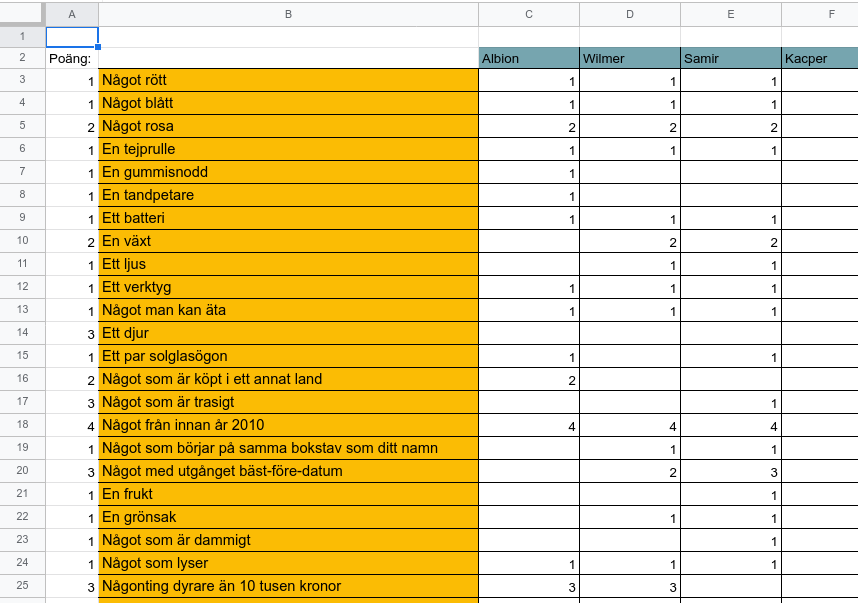
\includegraphics[scale=0.6]{./scav_list.png}
				\caption{Urdrag ur listan av objekt}
			\end{figure}

		\subsection{Moment 3 - Skribbl.io}
			Vid det sista momentet så ansåg vi att deltagarna stiftat en någorlunda bekantskap med varandra, så det kändes lämpligt att avsluta med något liter mer ledigt. Skribbl.io är en onlineversion av det populära spelet pictionary, vilket går ut på att en deltagare blir tillgiven ett ord att rita inför de andra deltagarna. De andra deltagarna är därefter menade att försöka gissa vilket ord deltagaren försöker rita. Olika mycket poäng tillskrivs de deltagare som gissar rätt beroende på hur snabba de var med sina respektiva gissningar, och efter en viss tid så presenteras rätt svar varpå turen går över till en ny deltagare att rita ett ord.\\

			Motiveringen bakom den här övningen var i huvudsak att det kändes som ett ganska lättsamt och okomplicerat sätt att avrunda dagen på.

		\subsection{Slutsatser Övning 1}
			Till största del är jag väldigt nöjd över vår planering samt utförande av övning. Till en början var stämningen lite stel i det första momentet, då det mestadels bara var en deltagare som presenterade en gissning och att övriga deltagare höll med, men emellanåt så skedde mindre debatter om vilket påstående som var en lögn egentligen. De flesta deltagare kändes investerade i de två resterande momenten som övningen erbjöd, vilket bidrog med en väldigt god stämmning. Den enda tabbe vi upplevde under övningens gång var hur en deltagare vid det första momentet hade med sig påståendet: ''Jag har haft Corona'' Det skedde därefter en väldigt kortfattad diskussion om att en deltagare fått se en nära släkting bli smittad av Covid-19, med kommentaren att ''sådana saker inte är något att skämta om'' Lyckligtvis så desarmerades vad som hade kunnat bli en mindre konflikt väldigt snabbt, men det var ändå ett missöde som skedde under övningens gång. Jag vet egentligen inte hur man bäst hade kunnat förutspå ett scenario i stil med detta, då den största boven egentligen känns som slump och eventuell oförsiktighet å deltagarnas vägnar, men man skulle ha kunnat gå ut med något meddelande i stil med att ''lämna diskussioner om den rådande pandemin utanför övningen'' (eller liknande). Liknande dilemman uppstådde aldrig senare, förmodligen för att gruppen hädanefter hade en bättre förståelse för varandras gränser låg.
	\section{Övning 2 - Kravfångst}
		Den andra övningen gick istället ut på att identifiera diverse krav på projektgruppens idé. Att göra det här till en gruppövning kan underlätta gruppens enighet gällande vad själva produkten handlar om, samt vad som är viktigt och mindre viktigt gällande deras modell om produkten.

		\subsection{Introduktion}
			För att öppna gruppmötet så gick vi kortfattat igenom dagens agenda samt vad syftet med just denna övning var. Vi beskrev, som ovan, att när övningen är klar så bör det finnas en mer enad bild av vad produkten innebär för gruppen. 

		\subsection{Moment 1 - Mentimeter}
			Därefter bjuds samtliga gruppmedlemmar in till att skapa en mentimeter tillsammans. Tanken med mentimetern är att man ska kunna brainstorma diverse tankar gällande vad som är åtråvärt gällande produkten. Vid det här stadiet ombads gruppmedlemmarna att ta med alla möjliga krav de kunde tänka på, att tänka utanför boxen helt enkelt.

			\begin{figure}[!h]
				\begin{center}
				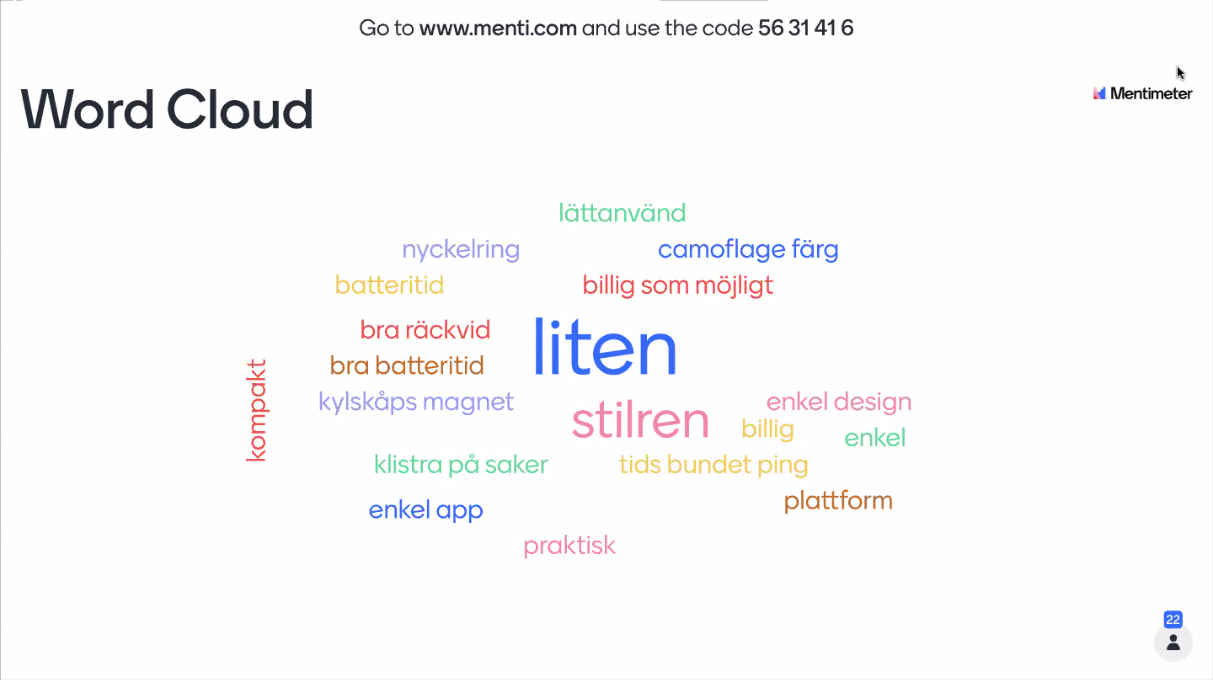
\includegraphics[scale=0.3]{./mentimeter.png}
				\caption{Det word cloud gruppen producerade}
				\end{center}
			\end{figure}
		\subsection{Moment 2 - User stories}
			Efter att gruppen börjat få igång hjärnkontoret så introducerades dem till konceptet av ''user stories''. En user story är en ganska informell formulering av vilka förväntningar en slutanvändare förväntas ha om produkten. Kortfattade exempel presenterades, i stil med: ''Som facebookanvändare vill jag kunna läsa meddelanden''. Deltagarna blev även tillgivna en enklare mall de kan förhålla sig till.

			\begin{figure}[h!]
				\begin{center}
				Som en \textbf{<konsument>} vill jag kunna \textbf{<funktion>}
				\end{center}
			\end{figure}

			Gruppen delades därefter in i mindre grupper beroende på vilket program de gick, med uppgift att formulera olika user stories en slutanvändare skulle kunna formulera. Tanken bakom att dela in dem beroende på program var att de på så vis skulle komma på mer nischade scenarion som var mer relevanta för deras utbildning. Exempelvis kanske gruppmedlemmar som går datateknik är mer intresserad av tekniska krav, medans en designstudent kanske intresserar sig mer för estetiska eller formmässiga krav. Efter ett antal minuter så förenades gruppen åter för att redovisa de user stories som producerats.\\

			När alla user stories presenterats så delades gruppen upp ytterligare en gång, den här gången var uppgiften istället att rangordna majoriteten av de olika krav som producerats i en MoSCoW lista. En MoSCoW lista är ett sätt att rangordna krav/behov på. Krav delas då in i Skallkrav (Must), Börkrav (Should), Bra att ha-krav (Could) eller Onödigt att ha-krav (Won't). Tanken med uppdelningen den här gången var istället att grupperna skulle ha så spridda åsikter som möjligt, så att de kravlistorna som producerades nu skulle bli så nyanserade som möjligt åsiktsmässigt. Vi försökte därför att placera gruppmedlemmar med gruppmedlemmar som inte gick samma program som dem själva. Även här blev de tilldelad en enklare mall med de olika kravnivåerna upplistade som de kunde förhålla sig till.\\

			Vi ville därefter egentligen slå samman kravlistorna en till gång, så att gruppen fick en slutgiltig kravlista de alla kunde vara eniga om. Dessvärre så hade klockan sprungit iväg en bra bit vid det här stadiet, så vi lämnade den övningen upp till gruppen att kika på ifall tid och intresse fanns.

			\subsection{Slutsatser Övning 2}

				Återigen så anser jag att övningen i dess helhet var lyckad, med några anmärkningar. I efterhand tror jag att det varit bättre om tidsuppdelningen skötts snyggare, så att vi hunnit med allting vi planerat. Jag är annars väldigt nöjd över planeringen av upplägget, framförallt våra motiveringar till de olika gruppindelningarna.\\

				Vid delmomentet då deltagarna ombeddes författa user stories så tolkade en grupp konceptet väldigt ordagrannt, och redovisade därför användarrecensioner de själva konstruerat som beskrev vad fiktiva användare hade för åsikter om produkten. Det här hade kanske kunnat förebyggas genom att förklara konceptet \emph{ännu} tydligare, eller genom att gå laget runt och be alla redovisa en user story innan man genomförde gruppindelningen, men i slutändan var det ändå ingen skada skedd, då det fanns mer än tillräckligt antal user stories att bygga krav av.

	\section{Övning 3 - Erfarenhetsmöte}
	\section{Övning 4 - Valfritt}
\end{document}
